%\documentclass{article}


\documentclass[a4paper]{article}
\usepackage[utf8]{inputenc}
\usepackage[12pt]{extsizes}
\usepackage{amsmath,amsthm,amssymb}
\usepackage[hidelinks]{hyperref} 
\usepackage[warn]{mathtext}
\usepackage[T1,T2A]{fontenc}
\usepackage[utf8]{inputenc}
\usepackage[english,russian]{babel}
\usepackage{tocloft}
\linespread{1.5}
\usepackage{indentfirst}
\usepackage{setspace}
%\полуторный интервал
\onehalfspacing

\newcommand{\RomanNumeralCaps}[1]
    {\MakeUppercase{\romannumeral #1}}

\usepackage{amssymb}

\usepackage{graphicx, float}
\graphicspath{{pictures/}}
\DeclareGraphicsExtensions{.pdf,.png,.jpg}
\usepackage[left=25mm,right=1cm,
    top=2cm,bottom=20mm,bindingoffset=0cm]{geometry}
\renewcommand{\cftsecleader}{\cftdotfill{\cftdotsep}}

%\addto\captionsrussian{\renewcommand{\contentsname}{СОДЕРЖАНИЕ}}
%\addto\captionsrussian{\renewcommand{\listfigurename}{СПИСОК ИЛЛЮСТРАЦИЙ}}

\usepackage{fancyhdr}
\usepackage[nottoc]{tocbibind}

\fancypagestyle{plain}{
\fancyhf{}
\renewcommand{\headrulewidth}{0pt}
\fancyhead[R]{\thepage}
}

\usepackage{blindtext}
\pagestyle{myheadings}
\usepackage{hyperref}

\begin{document}
\begin{titlepage}
  \begin{center}
    \large
    Санкт-Петербургский политехнический университет Петра Великого
    
    Институт прикладной математики и механики
    
    \textbf{Высшая школа прикладной математики и вычислительной физики}
    \vfill
    \textsc{\textbf{\large{Отчёт по лабораторной работе №3}}}\\[5mm]
     по дисциплине\\ <<Математическая статистика>>\\
\end{center}

\vfill

\begin{tabular}{l p{140} l}
Выполнила студентка \\группы 3630102/80401 && Мамаева Анастасия Сергеевна \\
\\
Проверил\\Доцент, к.ф.-м.н.& \hspace{0pt} &   Баженов Александр Николаевич \\\\
\end{tabular}

\hfill \break
\hfill \break
\begin{center} Санкт-Петербург \\2021 \end{center}
\thispagestyle{empty}
\end{titlepage}
\newpage
\newpage
\begin{center}
    \setcounter{page}{2}
    \tableofcontents
\end{center}
\newpage
\begin{center}
    \setcounter{page}{3}
    \listoffigures
\end{center}

\newpage
\section {Постановка задачи}
\noindent Для 5 распределений:
\begin{enumerate}
	\item $N(x, 0, 1)$ -- нормальное распределение
	\item $C(x, 0, 1)$ -- распределение Коши
	\item $L(x, 0, \frac{1}{\sqrt{2}})$ -- распределение Лапласа 
	\item $P(k, 10)$ -- распределение Пуассона
	\item $U(x, -\sqrt{3}, \sqrt{3})$ -- расномерное распределение
\end{enumerate}
Сгенерировать выборки размером 20 и 100 элементов.
Построить для них боксплот Тьюки.
Для каждого распределения определить долю выбросов экспериментально (сгенерировав выборку, соответствующую распределению 1000 раз, и вычислив среднюю долю выбросов) и сравнить с результатами, полученными теоретически.


\section {Теория}
\subsection{Боксплот Тьюки}
	\subsubsection{Определение}
	\noindent Боксплот (англ. box plot) — график, использующийся в описательной статистике, компактно изображающий одномерное распределение вероятностей
	
	\subsubsection{Описание}
	\noindent Такой вид диаграммы в удобной форме показывает медиану, нижний и верхний квартили и выбросы. Несколько таких ящиков можно нарисовать бок о бок, чтобы визуально сравнивать одно распределение с другим; их можно располагать как горизонтально, так и вертикально. Расстояния между различными частями ящика позволяют определить степень разброса (дисперсии) и асимметрии данных и выявить выбросы.
	
	\subsubsection{Построение}
	\noindent Границами ящика служат первый и третий квартили, линия в середине ящика — медиана. Концы усов — края статистически значимой выборки (без выбросов). Длину «усов» определяют разность первого квартиля и полутора межквартильных расстояний и сумма третьего квартиля и полутора межквартильных расстояний. Формула имеет вид
	\begin{equation}
	\label{mouns}
	{X_1 = Q_1-} \frac{3}{2}{(Q_3 - Q_1)},   {X_2 = Q_3+} \frac{3}{2}{(Q_3 - Q_1)}
	\end{equation}
	где $X_1$ — нижняя граница уса, $X_2$ — верхняя граница уса, $Q_1$ — первый квартиль, $Q_3$ — третий квартиль. Данные, выходящие за границы усов (выбросы), отображаются на графике в виде маленьких кружков.
	
	
\subsection{Теоретическая вероятность выбросов}
	\noindent Встроенными средствами языка программирования Python в среде разработки PyCharm можно вычислить теоретические первый и третий квартили распределений ($Q_1^T$ и $Q_3^T$ соответственно). По формуле \eqref{mouns} можно вычислить теоретические нижнюю и верхнюю границы уса ($X_1^T$ и $X_2^T$ соответственно). Выбросами считаются величины x, такие что: 
	\begin{equation}
		\left[
		\begin{gathered}
		x < X_1^T \\
		x > X_2^T \\
		\end{gathered}
		\right.
	\end{equation}
	Теоретическая вероятность выбросов для непрерывных распределений
	\begin{equation}
		P_B^T = P(x<X_1^T) + P(x>X_2^T)=F(X_1^T) + (1-F(X_2^T))
	\end{equation}
	где $F(X)=P(x\leq{X})$ - функция распределения.
	Теоретическая вероятность выбросов для дискретных распределений
	\begin{equation}
		P_B^T = P(x<X_1^T)+P(x>x_2^T)=(F(X_1^T)-P(x=X_1^T))+(1-F(X_2^T))
	\end{equation}
	где $F(X) = P(x\leq{X})$ - функция распределения
	
\section{Программная реализация}
\noindent Лабораторная работа выполнена на языке Python вресии 3.7 в среде разработки JupyterLab. Использовались дополнительные библиотеки:\\\\ 
1. scipy - статические распределения и функции\newline
2. seaborn - посроение графиков, визуализация \newline
3. matplotlib - построение графиков \newline
4. math - использование математических функций\\

\noindentВ приложении находится ссылка на GitHub репозиторий с исходныи кодом.

\section {Результаты} 
\subsection{Боксплот Тьюки}
\begin{figure}[H]
\center{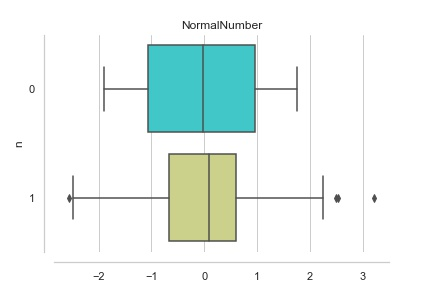
\includegraphics[scale=0.75]{NormalNumber.jpg}}
\label{fig:image}
\caption{Нормальное распределение} 
\end{figure}
	
\begin{figure}[H]
\center{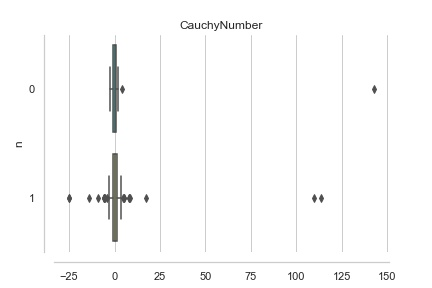
\includegraphics[scale=0.75]{CauchyNumber.jpg}}
\label{fig:image}
\caption{распределение Коши} 
\end{figure}

\begin{figure}[H]
\center{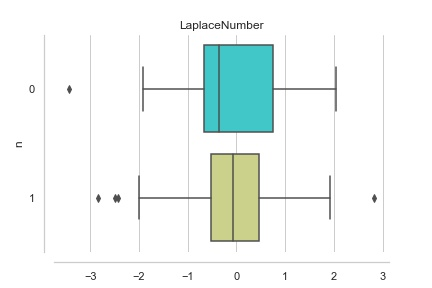
\includegraphics[scale=0.75]{LaplaceNumber.jpg}}
\label{fig:image}
\caption{распределение Лапласа} 
\end{figure}

\begin{figure}[H]
\center{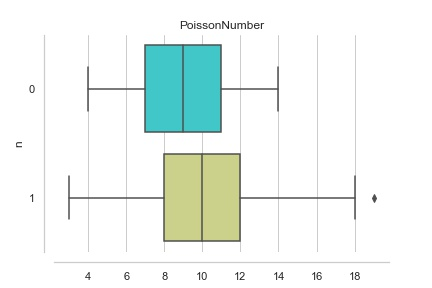
\includegraphics[scale=0.75]{PoissonNumber.jpg}}
\label{fig:image}
\caption{распределение Пуассона} 
\end{figure}

\begin{figure}[H]
\center{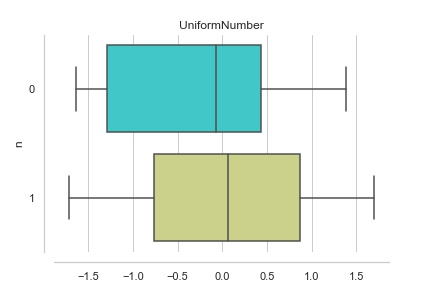
\includegraphics[scale=0.75]{UniformNumber.jpg}}
\label{fig:image}
\caption{равномерное распределение} 
\end{figure}							

\subsection{Доля выбросов}

\noindent Округление доли выбросов:\\
Выборка случайна, поэтому в качестве оценки рассеяния можно взять дисперсию пуассоновского потока:  $D_n \approx \sqrt{n}$\\
Доля $p_n = \frac{D_n}{n}=\frac{1}{\sqrt{n}}$\\
Доля $n=20: p_n=\frac{1}{\sqrt{20}}$ - примерно 0.2 или 20\% \\
Для $n=100: p_n=\frac{1}{\sqrt{100}}$ - примерно 0.1 или 10\% \\
Исходя из этого можно решить, сколько знаков оставлять в доле выброса.
\begin{table}[H]
		\centering
		\begin{tabular}[t]{lrr}
			\hline
			Выборка   &      Доля выбросов	& $P_B^T$		\\
			\hline
			Normal n=20   	&	0.023 		& 0.007		\\
			Normal n=100   	&  	0.014		& 0.007\\
			Cauchy n=20 	& 	0.152  		& 0.156		\\
			Cauchy n=100	&  	0.185 		& 0.156\\
			Laplace n=20	& 	0.080  		& 0.063	\\
			Laplace n=100	&   0.073 		& 0.063\\
			Poisson n=20	&	0.022 		& 0.008		\\
			Poisson n=100	&	0.015		& 0.008	\\
			Uniform n=20	&	0.003 		& 0		\\
			Uniform n=100	&	0 			& 0	\\
			\hline
		\end{tabular}
		\caption{Доля выбросов}
		\label{tab:normal}
	\end{table}


\subsection{Теоретическая вероятность выбросов}
	\begin{table}[H]
		\centering
		\begin{tabular}[t]{lrrrrr}
			\hline
			Распределение   &      $Q_1^T$	& $Q_3^T$ & $X_1^T$ & $X_2^T$ & $P_B^T$	\\
			\hline
			Нормальное распределение 	& -0.674& 0.674 & -2.698 	&  2.698 	& 0.007 \\
			Распределение Коши 			& -1	& 1		&  -4		& 4			& 0.156 \\
			Распределение Лапласа 		&-0.490	& 0.490	& -1.961	& 1.961		& 0.063\\
			Распределение Пуассона 		& 8		& 12	& 2			& 18		& 0.008 \\
			Равномерное распределение 	&-0.866 & 0.866	& -3.464 	& 3.464 	& 0	\\
			
			\hline
		\end{tabular}
		\caption{Теоретическая вероятность выбросов}
		\label{tab:normal}
	\end{table}
	
\section{Обсуждение}
\noindent По данным, приведенным в таблице, можно сказать, что чем больше выборка (в нашем случае для 100 элементов), тем ближе доля выбросов будет к теоретической оценке. Снова доля выбросов для распределения Коши значительно выше, чем для остальных распределений. Для распределений: нормального, Лапласа и Пуассона погрешность при большой выборке составила не более 2 процентов. При увеличении выборки равномерное распределение показывает стремительный рост к теоретической оценке - выбросы практически не наблюдаются.\\

\noindent Ящики с «усами» в удобной форме показывает многие важные характеристики выборки, такие как медиана, первый и третий квартили и другие. Исходня из которых можно делать выводы касательно природы входных данных, распределений.

\section{Приложение}

\noindent Код программы GitHub URL:\\
\newline https://github.com/Brightest-Sunshine/Math-Statistic-2021/blob/main/Lab3/Lab3.ipynb

\end{document}
